%%%%%%%%%%%%%%%%%%%%%%%%%%% asme2e.tex %%%%%%%%%%%%%%%%%%%%%%%%%%%%%%%
% Template for producing ASME-format articles using LaTeX            %
% Written by   Harry H. Cheng                                        %
%              Integration Engineering Laboratory                    %
%              Department of Mechanical and Aeronautical Engineering %
%              University of California                              %
%              Davis, CA 95616                                       %
%              Tel: (530) 752-5020 (office)                          %
%                   (530) 752-1028 (lab)                             %
%              Fax: (530) 752-4158                                   %
%              Email: hhcheng@ucdavis.edu                            %
%              WWW:   http://iel.ucdavis.edu/people/cheng.html       %
%              May 7, 1994                                           %
% Modified: February 16, 2001 by Harry H. Cheng                      %
% Modified: January  01, 2003 by Geoffrey R. Shiflett                %
% Use at your own risk, send complaints to /dev/null                 %
%%%%%%%%%%%%%%%%%%%%%%%%%%%%%%%%%%%%%%%%%%%%%%%%%%%%%%%%%%%%%%%%%%%%%%

%%% use twocolumn and 10pt options with the asme2e format
\documentclass[twocolumn,10pt]{asme2e}
\special{papersize=8.5in,11in}

%\usepackage{amsmath,amssymb,amsthm,amsfonts,amscd} % Some packages to write mathematics.
\usepackage{amsmath} % Some packages to write mathematics.
\usepackage{graphicx} 
%\usepackage{eucal} 	 		% Euler fonts
%\usepackage{verbatim}      	% Allows quoting source with commands.
%\usepackage{makeidx}       	% Package to make an index.
%\usepackage{psfig}         	% Allows inclusion of eps files.
%\usepackage{epsfig}        	% Allows inclusion of eps files.
%\usepackage{natbib}
%\usepackage{citesort}      	% 
%\usepackage{url}			% Allows good typesetting of web URLs.
%\usepackage{hyperref}
%\hypersetup{
    %colorlinks,
    %citecolor=black,
    %filecolor=black,
    %linkcolor=black,
    %urlcolor=black
%}
% \usepackage[backend=bibtex, style=alphabetic]{biblatex}
% \usepackage{courier}
% \usepackage[acronym, toc]{glossaries}
% \usepackage{listings}
%\usepackage{multirow} 		% multirow
%\usepackage{booktabs} 		% toprule, midrule, bottomrule
%\usepackage[caption=false]{subfig}% subcaptions for subfigures
%\usepackage{bmpsize}
%\usepackage{array}
%\usepackage{tabu}
%\usepackage[table]{xcolor}% http://ctan.org/pkg/xcolor
\usepackage{algorithm}
\usepackage{algpseudocode}
%\newcolumntype{L}[1]{>{\raggedright\let\newline\\\arraybackslash\hspace{0pt}}m{#1}}
%\newcolumntype{C}[1]{>{\centering\let\newline\\\arraybackslash\hspace{0pt}}m{#1}}
%\newcolumntype{R}[1]{>{\raggedleft\let\newline\\\arraybackslash\hspace{0pt}}m{#1}}
%\newtheorem{thm}{Theorem}[section]
%\newtheorem{cor}[thm]{Corollary}
%\newtheorem{lem}[thm]{Lemma}
%\newtheorem{prop}[thm]{Proposition}
%\newtheorem{ax}{Axiom}

%\theoremstyle{definition}
%\newtheorem{defn}{Definition}[section]

%\theoremstyle{remark}
%\newtheorem{rem}{Remark}[section]
%\newtheorem*{notation}{Notation}
\newcommand{\bs}[1]{\boldsymbol{#1}}
\newcommand{\latexe}{{\LaTeX\kern.125em2%
                      \lower.5ex\hbox{$\varepsilon$}}}
\newcommand{\amslatex}{\AmS-\LaTeX{}}
\chardef\bslash=`\\	% \bslash makes a backslash (in tt fonts)
			%	p. 424, TeXbook
\newcommand{\cn}[1]{\texttt{\bslash #1}}
\newcommand{\FT}{\mathcal{F}}
%% The class has several options
%  onecolumn/twocolumn - format for one or two columns per page
%  10pt/11pt/12pt - use 10, 11, or 12 point font
%  oneside/twoside - format for oneside/twosided printing
%  final/draft - format for final/draft copy
%  cleanfoot - take out copyright info in footer leave page number
%  cleanhead - take out the conference banner on the title page
%  titlepage/notitlepage - put in titlepage or leave out titlepage
%  
%% The default is oneside, onecolumn, 10pt, final

%%% Replace here with information related to your conference
\confshortname{OMAE2018}
\conffullname{Proceedings of the ASME 2018 37th International Conference on Ocean, Offshore and Arctic Engineering}

%%%%% for date in a single month, use
\confdate{17-22}
\confmonth{June}
%%%%% for date across two months, use
%\confdate{June 17-22}
\confyear{2018}
\confcity{Madrid}
\confcountry{Spain}

%%% Replace DETC2009/MESA-12345 with the number supplied to you 
%%% by ASME for your paper.
\papernum{OMAE2018/*****}

%%% You need to remove 'DRAFT: ' in the title for the final submitted version.
\title{DRAFT: Reliability Analysis of Floating Offshore Wind Turbine System Based on Polynomial Chaos Method}

%%% first author
\author{Jinsong Liu
    \affiliation{
	  Dept. of Civil, Arch. and Env. Engineering\\
	  University of Texas\\
	  Austin, Texas 78712\\
	  Email: Jinsongliu@utexas.edu
    }	
}

%%% second author
%%% remove the following entry for single author papers
%%% add more entries for additional authors
\author{Lance Manuel
    \affiliation{
	  Dept. of Civil, Arch. and Env. Engineering\\
	  University of Texas\\
	  Austin, Texas 78712\\
	  Email:lmanuel@mail.utexas.edu
    }
}

\begin{document}

\maketitle    

%%%%%%%%%%%%%%%%%%%%%%%%%%%%%%%%%%%%%%%%%%%%%%%%%%%%%%%%%%%%%%%%%%%%%%
\begin{abstract}
  {\it In reliability analysis, the objective is to evaluate the probability of failure of a system corresponding to a predefined reference period with respective to some performance functions. Various methods have been proposed to solve this problem efficiently, like Monte Carlo based sampling methods, approximation based FORM/SORM and surrogate models. However, the efficiency of these methods will decrease exponentially as the dimension of the problem increases. Even though the dimension-free property of Monte Carlo based methods are attractive, the slow convergence rate ($\propto 1/\sqrt{N}$) makes those approaches particularly inefficient. For an offshore system, the dimension of the random variables could easily be hundreds or thousands due to the existence of random phases when applying wind and/or wave spectrum. In this paper we propose to isolate the uncertainties induced due to environment random variables and random phases. Phase-conditioned meta-models, which are inexpensive to evaluate in contrast to the original model, are constructed based on Polynomial Chaos Expansion (PCE) under the framework of Uncertainty Quantification (UQ). The uncertainty of random phases will then be taken into account by bootstrapping from phase-conditioned meta-model pools. Since it is impossible to quantify the error made with surrogate model, this approach is first applied to a single DOF dynamic system with external wave loads. A few metrics are compared to assess the accuracy of this method against crude Monte Carlo method. The 50-year return loads of the SNL 13.2 MW semi-submersible floating offshore wind turbine model is eventually obtained with the constructed PCE surrogate models}
\end{abstract}

%%%%%%%%%%%%%%%%%%%%%%%%%%%%%%%%%%%%%%%%%%%%%%%%%%%%%%%%%%%%%%%%%%%%%%
\begin{nomenclature}
\entry{A}{You may include nomenclature here.}
\entry{$\alpha$}{There are two arguments for each entry of the nomemclature environment, the symbol and the definition.}
\end{nomenclature}

meta model for structural reliability and UQ \cite{sudret2012meta}

The accuracy of Polynomial chaos approximation \cite{field2004accuracy}

Three possible sources of discrepancy between simulation and experimental observations may be distinguished: Model inadequacy, Numerical Error and Input parameter uncertainty. Only the uncertainty in input parameters is addressed in this work. Probabilistic methods based on the representation of uncertain input parameters by random variables or random fields.

Non intrusive method, which only make use of a series of calls to the deterministic model. Also minimize the number of calls to the model.

Alternative is response surface method or metamodels. PCE: spectral methods provide a polynomial metamodel onto a basis that is well suited to post-processing in uncertainty and sensitivity analysis. Cons: Metamodeling reveal efficient and accurate for a moderate number of input parameters. Besides, Difficult in estimation of the approximation error, which directly depend on the goodness-of-fit of the metamodel. Reliable error estimate allow to design an adaptive refinement of the metamodel 

Let$ \left( \Omega, F, P \right)$ be a probability space, where $\Omega$ is the event space equipped with $\sigma$-algebra and probability measure $P$. Throughout this work, random variables are denoted by upper case letters $X(\omega): \Omega \to D_{X} \in R$, while their realizations are denoted by the corresponding lower case letters. Moreover, bold upper and lower case letters are used to denote random vectors and their realizations, respectively.

Standard methods for uncertainty propagation.

Statistical point view: Unbiased Estimator, However slow convergence rate. could be improved by LHS and QMC.
By definition, could also be viewed as integration. Quadrature rule could be applied. Curse of dimensionality. Could be improved by sparse quadrature schemes.



\section*{SDOF system}
Single DOF system defined by natural frequency and damping ratio. $\omega_n = 0.15 Hz, \zeta = 0.1$. 

\textbf{System transfer function as following}
\begin{equation*}
  H(\omega) = \frac{1}{\sqrt{(1 - \frac{\omega}{\omega_n})^2 + (2\zeta\frac{\omega}{\omega_n})^2}}
\end{equation*}

\textbf{External loads are assumed to be wave loads. JONSWAP wave spectrum is used as recommend by standard IEC 61400-3}

Pierson-Moskowitz (PM) spectrum $S_{PM}(\omega)$ is given by:
\begin{equation}
S_{PM}(\omega) = \frac{5}{16} \cdot H_s^2 \omega_p^4 \cdot \omega^{-5} \mathrm{exp}\left(-\frac{5}{4}\left( \frac{\omega}{\omega_p} \right)^{-4}\right)
  \label{eqn:Pierson-Moskowitz}
\end{equation}

where $\omega_p = 2\pi/T_p$ is the angular spectral peak frequency.

JONSWAP Spectrum:

\begin{equation}
  S_J(\omega) = A_\gamma S_{PM}(\omega) \gamma^{\mathrm{exp}\left[-0.5(\frac{\omega-\omega_p}{\sigma \cdot \omega_p})^2\right]}
  \label{eqn:JONSWAP}
\end{equation}
where $S_{PM}(\omega)$ is pierson-Moskowitz spectrum, $\gamma = 3.3$ is non-dimensional peak shape parameter. $\sigma$ is spectral width parameter, $\sigma = \sigma_a = 0.07$ for $\omega \leq \omega_p$ and $\sigma = \sigma_b = 0.09$ for $\omega > \omega_p$. $A_\gamma = 1 - 0.287 \mathrm{ln} (\gamma)$ is a normalizing factor. 

\begin{figure*}[]
  \centering
  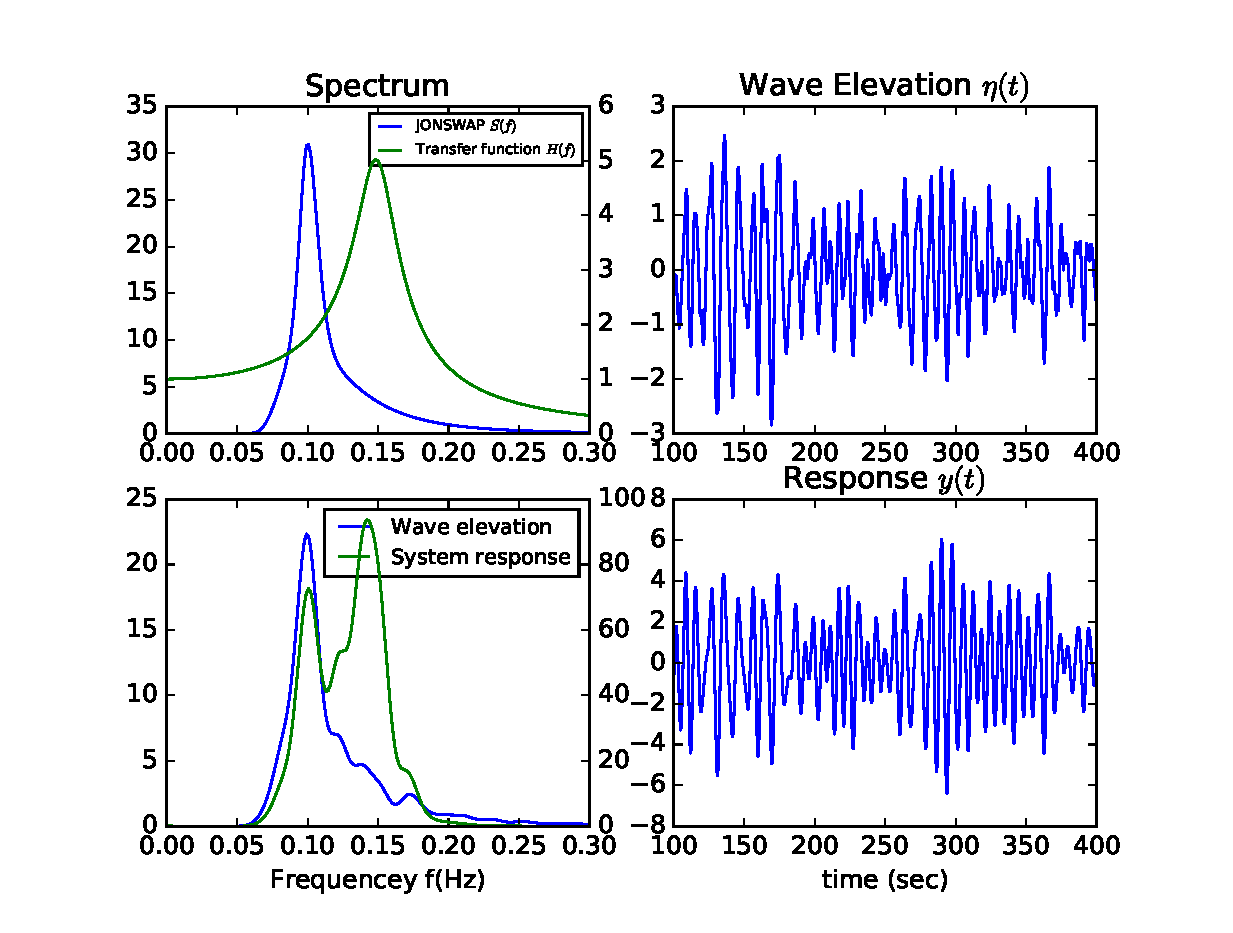
\includegraphics{Figures/SDOF.eps}
  \caption{SDOF sysmtem properties}
  \label{fig:SDOF_400}
\end{figure*}

\textbf{Check if the variance of system introduced due to random phases is comparable with wind turbine system.}

To achieve $10^{-6}$ failure probability with $CV_{p_f} \leq 10\%$, requires about $10^{8}$ simulations

\begin{table}[]
\centering
\caption{System variance indicator introuded by random phases}
\label{my-label}
\begin{tabular}{ccccccccc} \hline
  & \multicolumn{8}{c}{quantile of $F_{T_p | Hs}$}           \\ \hline
$H_s (m)$ & 0.1  & 0.2  & 0.3  & 0.4  & 0.5  & 0.6  & 0.7  & 0.8  \\ \hline
1     & 1.12 & 1.17 & 1.12 & 1.16 & 1.22 & 1.21 & 1.28 & 1.32 \\
2     & 1.16 & 1.32 & 1.27 & 1.26 & 1.45 & 1.17 & 1.4  & 1.25 \\
3     & 1.24 & 1.39 & 1.23 & 1.13 & 1.2  & 1.12 & 1.08 & 1.27 \\
4     & 1.3  & 1.21 & 1.24 & 1.29 & 1.29 & 1.28 & 1.1  & 1.47 \\
5     & 1.21 & 1.14 & 1.35 & 1.29 & 1.17 & 1.15 & 1.1  & 1.19 \\
6     & 1.11 & 1.2  & 1.22 & 1.23 & 1.12 & 1.26 & 1.32 & 1.13 \\
7     & 1.25 & 1.29 & 1.27 & 1.26 & 1.19 & 1.24 & 1.24 & 1.08 \\
8     & 1.1  & 1.19 & 1.25 & 1.27 & 1.2  & 1.16 & 1.33 & 1.17 \\
9     & 1.21 & 1.12 & 1.35 & 1.15 & 1.36 & 1.19 & 1.26 & 1.36 \\ \hline
\end{tabular}
\end{table}
\section{PCE Structural Reliability}

Xiu in \cite{xiu2002wiener} proposed and numerically demonstrated the optimal (exponential) convergence rate of each Wiener-Askey polynomial chaos expansion for its corresponding stochastic process. Idealy, if the independent variable $\zeta$ in the polynomials ${\Phi_i(\zeta)}$ belong to the basic types as shown in Wiener-Askey scheme, the exponential convergence rate could be achieved. However, like the Weilbull and Lognormal distributions used in the current research, we often encounter distributions of random inputs not listed. A transformation could be used to map the target random variables to basic random variables. 

The target is the 50-year return loads. Based on Possion process assumption etc, we can evalute the extreme loads based on the maximum load within simulation duration. If conditions ** meets, block maxima will follow generalized extreme value distributions.

Quantity of interest (QoI) could be defined as following


$y_{max} ^i$ represents the maximum response value of the $i^{th}$ simulation with duration 400 seconds, $i = 1, \dots 100$.  $\mathrm{max}\left\{ y_{max}^i \right\} / \mathrm{mean}\left\{  y_{max}^i \right\}  $ is selected to indicate the random phases variance. 

a standard uniform random variable is first chosen, $u \in U(0,1)$. The CDFs for physical random variable $\bs{x}$ and random variable $\bs{\zeta}$ chosen from the list are $F_{\bs{X}}$ and $F_{\bs{Z}}$. Then we can set $u = F_{\bs{X}}(x) = F_{\bs{Z}}(\zeta)$
Howver since we don't know what is the best for that distribution, this approximiation could be reasonable.

Random variables: $\bs{X}$, Environmental Random variables. $\bs{\Theta}$: Random phases. $Y = f(\bs{X}, \bs{\Theta})$ \iffalse $Y(t) = f(t,\bs{X}, \bs{\Theta})$ \fi : response with unknown marginal distribution $F_Y$. Note that $\bs{\Theta}$ and $\bs{X}$ are independent.
\begin{equation}
  \begin{aligned}
  \Pr \left( Y > y_0 \right) 
  &= \int \Pr \left( f(\bs{X} | \bs{\Theta}) > y_0 \right) f_{\bs{\Theta}}\left( \bs{\Theta} = \bs{\theta} \right) d \bs{\Theta} \\
%  &= \iint \Pr \left( Y > y_0 | \bs{\Theta} = \bs{\theta}, \bs{X} = \bs{x} \right) f_{\bs{\Theta}}\left( \bs{\Theta} = \bs{\theta} \right) f_{\bs{X}}(\bs{X} = \bs{x}) d \bs{\Theta} d \bs{X} \\
  &=\iint \Pr \left( f(\bs{x},\bs{\theta}) > y_0  \right) f_{\bs{X}}(\bs{X} = \bs{x}) d \bs{X} f_{\bs{\Theta}}\left( \bs{\Theta} = \bs{\theta} \right) d \bs{\Theta}   \\ 
  %&= \iint \Pr \left( y(\bs{X}) \right)
  \end{aligned}
  \label{eqn:Reli_PCE_WindTurbine}
\end{equation}

The idea to solve this problem is to seperate the uncertainty introduced by random phases and physical random variables. According to TurbSim, the random numbers generated by the pRNG are used to create random phases (one per frequency per grid point per wind component) for the velocity time series. The difficulty to quantify the phase uncertainties comes from the large dimensions and the dimension changes as we create or apply different wind model. In addition, we can bearly control the random phases unless we know the pRNG. Thus the following alternatives are proposed. Say, our goal is 50-year return loads and simulation duration is 1-hour. Our QoI can either be the block maxima (assumptions here like possion process; POT works here?) or the time series itself.

Define the maxima in duration $T$ is $y_{max}$. Then the QoI can be expressed with PCE as following:
\begin{equation}
  y_{max}^K (\bs{x} | \bs{\theta}) = \sum _{k=0}^K \alpha_k \Phi_k(\bs{u})
  \label{eqn:Block_maxima_PCE}
\end{equation}

If the QoI is the time series, then expression can be written as:
\begin{equation}
  y^K(\bs{x},t) = \sum _{k=0} ^ K \alpha_k (t) \Phi_k(\bs{u})
  \label{eqn:TimeSeries_PCE}
\end{equation}

The inner integral conditional on $\Theta$ in Eqn. \ref{eqn:Reli_PCE_WindTurbine} can be appxomiated as:

\begin{equation}
  \Pr \left( Y > y_0 | \Theta \right)  = \int \Pr \left( y_{max}^K (\bs{x}|\bs{\theta}) > y_0 \right) f_{\bs{X}} d \bs{X}
  \label{eqn:Reli_BM_PCE}
\end{equation}
Or

\begin{equation}
  \Pr \left( Y > y_0 | \Theta \right)  = \int \Pr \left( y^K (\bs{x},t|\bs{\theta}) > y_0 \right) f_{\bs{X}} d \bs{X}
  \label{eqn:Reli_TS_PCE}
\end{equation}

The next step is to account for the outer integral, sampling from $\Theta$ space. One critical question is then to choose the proper number of samples $N_\theta$ to represent the distribution as well as to quantify the uncertainty."Repeat for $N_\theta$ times with different $\theta$ samples. (need a metric to determine)

Once this step is done, the following algorithm could be used to estimate the 50-year return load.

number of samples(numSamples) = 50 year / T \\
\begin{algorithm}
  \begin{algorithmic}
	\For{ $i = 1 \colon \mathrm{numSamples}$}
	  \State $X_i \sim F_{\bs{X}}$
	  \State select $\bs{\theta}$ from pre-runned $\theta$ pool
	  \Comment{Can pick $\theta$ uniformly from $N_{\theta}$ samples or add weight based on sampling results}
	  \State $y_{max}^i = y_{max}^K (X_i, \theta)$
	\EndFor
	\State 50 year return load = $\mathrm{max } \left\{ y_{max}^i \right\}$
  \end{algorithmic}
\end{algorithm}

\begin{algorithm}
  \begin{algorithmic}
	\For{ $i = 1 \colon \mathrm{numSamples}$}
	  \State $X_i \sim F_{\bs{X}}$
	  \State select $\bs{\theta}$ from pre-runned $\theta$ pool
	  \Comment{Can pick $\theta$ uniformly from $N_{\theta}$ samples or add weight based on sampling results}
	  \State $y_{max}^i = \mathrm{max}\left\{y^K (X_i, t,\theta) \right\}$
	\EndFor
	\State 50 year return load = $\mathrm{max } \left\{ y_{max}^i \right\}$
  \end{algorithmic}
\end{algorithm}
The spacing between abstract and the text heading is two line spaces.  The primary text heading is  boldface in all capitals, flushed left with the left margin.  The spacing between the  text and the heading is also two line spaces.

Is the variance in SDOF model competible with wind turbine?
%%%%%%%%%%%%%%%%%%%%%%%%%%%%%%%%%%%%%%%%%%%%%%%%%%%%%%%%%%%%%%%%%%%%%%%
%\section*{INTRODUCTION}

%This article illustrates preparation of ASME paper using \LaTeX2\raisebox{-.3ex}{$\epsilon$}. The \LaTeX\  macro \verb+asme2e.cls+, the {\sc Bib}\TeX\ style file \verb+asmems4.bst+, and the template \verb+asme2e.tex+ that create this article are available on the WWW  at the URL address \verb+http://iel.ucdavis.edu/code/+. To ensure compliance with the 2003 ASME MS4 style guidelines  \cite{asmemanual}, you should modify neither the \LaTeX\ macro \verb+asme2e.cls+ nor the {\sc Bib}\TeX\ style file \verb+asmems4.bst+. By comparing the output generated by typesetting this file and the \LaTeX2\raisebox{-.3ex}{$\epsilon$} source file, you should find everything you need to help you through the preparation of ASME paper using \LaTeX2\raisebox{-.3ex}{$\epsilon$}. Details on using \LaTeX\ can be found in \cite{latex}. Instructions for submitting an electronic version of a paper via ftp for publication on CD-ROM or online  are given at the URL address \verb+http://www.asme.org/pubs/submittal.html+.

%%%%%%%%%%%%%%%%%%%%%%%%%%%%%%%%%%%%%%%%%%%%%%%%%%%%%%%%%%%%%%%%%%%%%%%
%\section*{VERY VERY VERY VERY VERY VERY VERY VERY LONG HEADING}

%If the heading should run into more than one line, the run-over is flush left.

%%%%%%%%%%%%%%%%%%%%%%%%%%%%%%%%%%%%%%%%%%%%%%%%%%%%%%%%%%%%%%%%%%%%%%%
%\subsection*{Second-Level Heading}

%The next level of heading is boldface with upper and lower case letters. The heading is flushed left with the left margin. The spacing to the next heading is two line spaces.

%%%%%%%%%%%%%%%%%%%%%%%%%%%%%%%%%%%%%%%%%%%%%%%%%%%%%%%%%%%%%%%%%%%%%%%
%\subsubsection*{Third-Level Heading.}

%The third-level of heading follows the style of the second-level heading, but it is indented and followed by a period, a space, and the start of corresponding text.

%%%%%%%%%%%%%%%%%%%%%%%%%%%%%%%%%%%%%%%%%%%%%%%%%%%%%%%%%%%%%%%%%%%%%%
%\section*{PAPER NUMBER}

%ASME assigns each accepted paper with a unique number. Replace {\bf DETC98/DAC-1234} in the input file preamble (the location will be obvious) with the paper number supplied to you  by ASME for your paper.


%%%%%%%%%%%%%%%%%%%%%%%%%%%%%%%%%%%%%%%%%%%%%%%%%%%%%%%%%%%%%%%%%%%%%%%
%\section*{USE OF SI UNITS}

%An ASME paper should use SI units.  When preference is given to SI units, the U.S. customary units may be given in parentheses or omitted. When U.S. customary units are given preference, the SI equivalent {\em shall} be provided in parentheses or in a supplementary table. 
%%%%%%%%%%%%%%%%%%%%%%%%%%%%%%%%%%%%%%%%%%%%%%%%%%%%%%%%%%%%%%%%%%%%%%%
%\section*{MATHEMATICS}

%Equations should be numbered consecutively beginning with (1) to the end of the paper, including any appendices.  The number should be enclosed in parentheses and set flush right in the column on the same line as the equation.  An extra line of space should be left above and below a displayed equation or formula. \LaTeX\ can automatically keep track of equation numbers in the paper and format almost any equation imaginable. An example is shown in Eqn.~(\ref{eq_ASME}). The number of a referenced equation in the text should be preceded by Eqn.\ unless the reference starts a sentence in which case Eqn.\ should be expanded to Equation.

%\begin{equation}
%f(t) = \int_{0_+}^t F(t) dt + \frac{d g(t)}{d t}
%\label{eq_ASME}
%\end{equation}

%%%%%%%%%%%%%%%%%%%%%%%%%%%%%%%%%%%%%%%%%%%%%%%%%%%%%%%%%%%%%%%%%%%%%%%
%\section*{FIGURES AND TABLES}

%All figures should be positioned at the top of the page where possible.  All figures should be numbered consecutively and captioned; the caption uses all capital letters, and centered under the figure as shown in Fig.~\ref{figure_ASME}. All text within the figure should be no smaller than 7~pt. There should be a minimum two line spaces between figures and text. The number of a referenced figure or table in the text should be preceded by Fig.\ or Tab.\ respectively unless the reference starts a sentence in which case Fig.\ or Tab.\ should be expanded to Figure or Table.


%%%%%%%%%%%%%%%%%%%%%%%%%%%%%%%%%%%%%%%%%%%%%%%%%%%%%%%%%%%%%%%%%%%%%%%
%%%%%%%%%%%%%%%%% begin figure %%%%%%%%%%%%%%%%%%%
%\begin{figure}[t]
%\begin{center}
%\setlength{\unitlength}{0.012500in}%
%\begin{picture}(115,35)(255,545)
%\thicklines
%\put(255,545){\framebox(115,35){}}
%\put(275,560){Beautiful Figure}
%\end{picture}
%\end{center}
%\caption{THE FIGURE CAPTION USES CAPITAL LETTERS.}
%\label{figure_ASME} 
%\end{figure}
%%%%%%%%%%%%%%%%% end figure %%%%%%%%%%%%%%%%%%% 
%%%%%%%%%%%%%%%%%%%%%%%%%%%%%%%%%%%%%%%%%%%%%%%%%%%%%%%%%%%%%%%%%%%%%%%


%%%%%%%%%%%%%%%%%%%%%%%%%%%%%%%%%%%%%%%%%%%%%%%%%%%%%%%%%%%%%%%%%%%%%%%
%%%%%%%%%%%%%%%% begin table   %%%%%%%%%%%%%%%%%%%%%%%%%%
%\begin{table}[t]
%\caption{THE TABLE CAPTION USES CAPITAL LETTERS, TOO.}
%\begin{center}
%\label{table_ASME}
%\begin{tabular}{c l l}
%& & \\ % put some space after the caption
%\hline
%Example & Time & Cost \\
%\hline
%1 & 12.5 & \$1,000 \\
%2 & 24 & \$2,000 \\
%\hline
%\end{tabular}
%\end{center}
%\end{table}
%%%%%%%%%%%%%%%%% end table %%%%%%%%%%%%%%%%%%% 
%%%%%%%%%%%%%%%%%%%%%%%%%%%%%%%%%%%%%%%%%%%%%%%%%%%%%%%%%%%%%%%%%%%%%%%

%All tables should be numbered consecutively and  captioned; the caption should use all capital letters, and centered above the table as shown in Table~\ref{table_ASME}. The body of the table should be no smaller than 7 pt.  There should be a minimum two line spaces between tables and text.

%%%%%%%%%%%%%%%%%%%%%%%%%%%%%%%%%%%%%%%%%%%%%%%%%%%%%%%%%%%%%%%%%%%%%%%%
%\section*{FOOTNOTES\protect\footnotemark}
%\footnotetext{Examine the input file, asme2e.tex, to see how a footnote is given in a head.}

%Footnotes are referenced with superscript numerals and are numbered consecutively from 1 to the end of the paper\footnote{Avoid footnotes if at all possible.}. Footnotes should appear at the bottom of the column in which they are referenced.


%%%%%%%%%%%%%%%%%%%%%%%%%%%%%%%%%%%%%%%%%%%%%%%%%%%%%%%%%%%%%%%%%%%%%%%%
%\section*{CITING REFERENCES}

%%%%%%%%%%%%%%%%%%%%%%%%%%%%%%%%%%%%%%%%%%%%%%%%%%%%%%%%%%%%%%%%%%%%%%%
%The ASME reference format is defined in the authors kit provided by the ASME.  The format is:

%\begin{quotation}
%{\em Text Citation}. Within the text, references should be cited in  numerical order according to their order of appearance.  The numbered reference citation should be enclosed in brackets.
%\end{quotation}

%The references must appear in the paper in the order that they were cited.  In addition, multiple citations (3 or more in the same brackets) must appear as a `` [1-3]''.  A complete definition of the ASME reference format can be found in the  ASME manual \cite{asmemanual}.

%The bibliography style required by the ASME is unsorted with entries appearing in the order in which the citations appear. If that were the only specification, the standard {\sc Bib}\TeX\ unsrt bibliography style could be used. Unfortunately, the bibliography style required by the ASME has additional requirements (last name followed by first name, periodical volume in boldface, periodical number inside parentheses, etc.) that are not part of the unsrt style. Therefore, to get ASME bibliography formatting, you must use the \verb+asmems4.bst+ bibliography style file with {\sc Bib}\TeX. This file is not part of the standard BibTeX distribution so you'll need to place the file someplace where LaTeX can find it (one possibility is in the same location as the file being typeset).

%With \LaTeX/{\sc Bib}\TeX, \LaTeX\ uses the citation format set by the class file and writes the citation information into the .aux file associated with the \LaTeX\ source. {\sc Bib}\TeX\ reads the .aux file and matches the citations to the entries in the bibliographic data base file specified in the \LaTeX\ source file by the \verb+\bibliography+ command. {\sc Bib}\TeX\ then writes the bibliography in accordance with the rules in the bibliography .bst style file to a .bbl file which \LaTeX\ merges with the source text.  A good description of the use of {\sc Bib}\TeX\ can be found in \cite{latex, goosens} (see how 2 references are handled?).  The following is an example of how three or more references \cite{latex, asmemanual,  goosens} show up using the \verb+asmems4.bst+ bibliography style file in conjunction with the \verb+asme2e.cls+ class file. Here are some more \cite{art, blt, ibk, icn, ips, mts, mis, pro, pts, trt, upd} which can be used to describe almost any sort of reference.

%% Here's where you specify the bibliography style file.
%% The full file name for the bibliography style file 
%% used for an ASME paper is asmems4.bst.
\bibliographystyle{asmems4}


%%%%%%%%%%%%%%%%%%%%%%%%%%%%%%%%%%%%%%%%%%%%%%%%%%%%%%%%%%%%%%%%%%%%%%%
%\begin{acknowledgment}
%Thanks go to D. E. Knuth and L. Lamport for developing the wonderful word processing software packages \TeX\ and \LaTeX. I also would like to thank Ken Sprott, Kirk van Katwyk, and Matt Campbell for fixing bugs in the ASME style file \verb+asme2e.cls+, and Geoff Shiflett for creating 
%ASME bibliography stype file \verb+asmems4.bst+.
%\end{acknowledgment}

%%%%%%%%%%%%%%%%%%%%%%%%%%%%%%%%%%%%%%%%%%%%%%%%%%%%%%%%%%%%%%%%%%%%%%%
%% The bibliography is stored in an external database file
%% in the BibTeX format (file_name.bib).  The bibliography is
%% created by the following command and it will appear in this
%% position in the document. You may, of course, create your
%% own bibliography by using thebibliography environment as in
%%
%% \begin{thebibliography}{12}
%% ...
%% \bibitem{itemreference} D. E. Knudsen.
%% {\em 1966 World Bnus Almanac.}
%% {Permafrost Press, Novosibirsk.}
%% ...
%% \end{thebibliography}

%% Here's where you specify the bibliography database file.
%% The full file name of the bibliography database for this
%% article is asme2e.bib. The name for your database is up
%% to you.
\bibliography{../PhD_Dissertation/JinsongLiuBib.bib}

%%%%%%%%%%%%%%%%%%%%%%%%%%%%%%%%%%%%%%%%%%%%%%%%%%%%%%%%%%%%%%%%%%%%%%%

%\appendix       %%% starting appendix

%\section*{Appendix A: Head of First Appendix}
%Avoid Appendices if possible.

%%%%%%%%%%%%%%%%%%%%%%%%%%%%%%%%%%%%%%%%%%%%%%%%%%%%%%%%%%%%%%%%%%%%%%
%\section*{Appendix B: Head of Second Appendix}
%\subsection*{Subsection head in appendix}
%The equation counter is not reset in an appendix and the numbers will
%follow one continual sequence from the beginning of the article to the very end as shown in the following example.
%\begin{equation}
%a = b + c.
%\end{equation}


\section{Model Selection}
Goals in model selection include: accurate predictions, interpretable models(determining which predictors are meaningful), stability(small changes in the data should not result in large changes in either the subset of predictors used, the associated coefficients, or the predictors), and avoiding bias in the hypothesis tests during or after variable selection.

Stepwise regression and All-subsets regression:

\end{document}
